\documentclass[9pt]{beamer}
\usepackage{silence}
\WarningFilter{beamerthememetropolis}{You need to compile with XeLaTeX or LuaLaTeX to use the Fira fonts}
\usetheme[titleformat = smallcaps, block = fill, progressbar = frametitle]{metropolis}
\title{\Huge Methods of Linear Algebra}
%---------------------------------%
% PACKAGES
%---------------------------------%
% Input encoding.
\usepackage[utf8]{inputenc} % For accents in spanish: transforms "á" into "\'a"
\usepackage[T1]{fontenc} % Output encoding. Use to avoid silly problems on the output.
                         % See: http://tex.stackexchange.com/questions/664/why-should-i-use-usepackaget1fontenc
\usepackage[sfdefault]{FiraSans}
\usepackage{FiraMono}
% AMS packages
\usepackage{amsmath}
\usepackage{amsfonts}
\usepackage{amssymb}
\usepackage{amsthm}
% Matrices
\usepackage{mathtools}
\newcommand{\verteq}{\rotatebox{90}{$\,=$}}
\usepackage{gauss}
% Customization for augmented matrices; 
% see https://tex.stackexchange.com/questions/146723/how-to-typeset-row-operations-on-augmented-matrix
% Patch gauss macros for doing their work in `align'
% and other amsmath environments; see http://tex.stackexchange.com/questions/146532/
\usepackage{etoolbox}
\makeatletter
\patchcmd\g@matrix
    {\vbox\bgroup}
    {\vbox\bgroup\normalbaselines} % restore the standard baselineskip
    {}{}
\makeatother
\newcommand{\BAR}{%
    \hspace{-\arraycolsep}%
    \strut\vrule % the `\vrule` is as high and deep as a strut
    \hspace{-\arraycolsep}%
}
% Math blackboard font
\usepackage{bbm}
% Fonts
\usepackage{lmodern} 
% \usepackage[sfdefault]{FiraSans}
\usepackage[normalem]{ulem}
\usepackage{eulervm}
% Graphics
\usepackage{graphicx} 
\usepackage{float}
\usepackage{subcaption}
\usepackage{wrapfig}
\usepackage{animate}
\usepackage{caption}
% Algorithms
\usepackage[ruled]{algorithm2e}
\newcommand{\lIfElse}[3]{\lIf{#1}{#2 \textbf{else}~#3}}
% Boxes
\usepackage[most]{tcolorbox}
% For reference enumerations lists
\usepackage{enumitem}
% \setlist{labelwidth = \widthof{0.}, leftmargin = {\labelwidth+\labelsep}, 
%         rightmargin = \leftmargin} % Setting left marging = right marging in itemize envirnment
% Import icons
\usepackage{fontawesome}
% Hyperlink
\usepackage{hyperref}
\hypersetup{
	final,
    bookmarksnumbered=true,
    bookmarksopen=true,
    bookmarksopenlevel=0,
    unicode=false,          % non-Latin characters in Acrobat?s bookmarks
    pdftoolbar=true,        % show Acrobat?s toolbar?
    pdfmenubar=true,        % show Acrobat?s menu?
    pdffitwindow=false,     % window fit to page when opened
    pdftitle={Introduction to Mathematics},    % title
    pdfdisplaydoctitle=true, %display document title instead of file name in title bar
    pdftoolbar=true,
    pdfmenubar=true,
    pdflang={English},
    pdfauthor={Abel Guada Azze},     % author
    pdfsubject={Introduction to Mathematics},   % subject of the document
    pdfcreator={Abel Guada Azze},   % creator of the document
    pdfproducer={Abel Guada Azze}, % producer of the document
    pdfkeywords={Mathematics} {introduction}, % list of keywords
    pdfnewwindow=true,      % links in new window
    breaklinks=true,
    hidelinks,
    colorlinks,
    linkcolor=black,          % color of internal links (change box color with linkbordercolor)
    citecolor=black,        % color of links to bibliography
    filecolor=cyan,      % color of file links
    urlcolor=magenta           % color of external links
}
%----------------------------------- Tikz
\usepackage{tikz}
\usepackage{pgfplots}
% \pgfplotsset{compat=1.18}
% \usepackage{tkz-euclide}
\usetikzlibrary{shapes,arrows.meta,matrix,positioning,calc}
\newcommand{\tikzmark}[1]{\tikz[baseline,remember picture] \coordinate (#1) {};}
% ---------- Helpers: 2-set and 3-set Venns ----------
% \VennTwoCounts{LabelA}{LabelB}{onlyA}{both}{onlyB}{Neither}{Universe}
\newcommand{\VennTwoCounts}[7]{%
  \begin{tikzpicture}[scale=1.0,baseline=(current bounding box.center)]
    \def\r{1.8}   % circle radius (cm)
    \def\dx{2.35} % distance between centres (cm)
    \def\pad{0.60} % padding between circles and rectangle (cm)

    \coordinate (A) at (0,0);
    \coordinate (B) at (\dx,0);

    % Universe rectangle (outline only)
    \draw[line width=.8pt, rounded corners=2pt]
      ($(A)+(-\r-\pad,-\r-\pad)$) rectangle ($(B)+(\r+\pad,\r+\pad)$);

    % Set fills + outlines
    \fill[black!8] (A) circle (\r);
    \fill[black!8] (B) circle (\r);
    \draw[line width=.8pt] (A) circle (\r);
    \draw[line width=.8pt] (B) circle (\r);

    % Universe label (top-left inside the box)
    \node[font=\scriptsize,anchor=north west]
      at ($(A)+(-\r-\pad+0.12,\r+\pad-0.12)$) {#7};

    % Set labels
    \node[font=\small\bfseries] at ($(A)+(0,0.68*\r)$) {#1};
    \node[font=\small\bfseries] at ($(B)+(0,0.68*\r)$) {#2};

    % Counts
    \node[font=\small] at ($ (A)+(-0.60*\r,-0.05*\r) $) {#3}; % only A
    \node[font=\small] at ($ .5*(A)+.5*(B) $) {#4};           % both
    \node[font=\small] at ($ (B)+(0.60*\r,-0.05*\r) $) {#5};  % only B
    \node[font=\small]
      at ($ (B)+(\r+0.3*\pad,0.78*\r) $) {#6};                % outside
  \end{tikzpicture}%
}


%---------------------------------%
% Biblio
%---------------------------------%

%---------------------------------%
% SETTINGS
%---------------------------------%
% displays sections and subsections numbered in the TOC
\setbeamertemplate{section in toc}[sections numbered]
% \setbeamertemplate{subsection in toc}[subsections numbered]
% gets rid of bottom navigation bars
\setbeamertemplate{footline}{}
% gets rid of bottom navigation symbols
\setbeamertemplate{navigation symbols}{}
% sets images' path
\graphicspath{{img/}}
% resets footnote counter at the beginning of each section
\AtBeginEnvironment{frame}{\setcounter{footnote}{0}}
% beamer margins
\setbeamersize
{
    text margin left=3mm,
    text margin right=3mm,
    % sidebar width left=.0cm,
    % sidebar width right=.0cm,
    % description width,
    % description width of=,
    % mini frame size=,
    % mini frame offset
}
% redefines block environment to add small space between title and content
\let\oldblock\block
\let\endoldblock\endblock
\renewenvironment{block}[1]
    {\begin{oldblock}{#1}
        \vspace{0.1cm}
    }
    { 
    \end{oldblock}
    }

%---------------------------------%
% SETTINGS
%---------------------------------%
%---------------------------------%
% TITLE PAGE
%---------------------------------%
\setbeamertemplate{title page}{
    \vspace{-0.4cm}
    
    \textcolor{CUNEForange}{\rule{\textwidth}{0.05cm}}
    \vspace{-0.65cm}
    
    \begin{minipage}{0.2\textwidth}
        \includegraphics[width = 2.0cm]{Logo-CUNEF.png}
    \end{minipage}
    \begin{minipage}{0.7\textwidth}
        
        \quad \Huge \usebeamertemplate*{title}
        
    \end{minipage}    
    \vspace{-0.25cm}
    
    \textcolor{CUNEForange}{\rule{\textwidth}{0.05cm}}
    \vspace{1.5cm}

    \begin{minipage}{0.075\textwidth}
        
    \end{minipage}\hfill\textcolor{CUNEForange}{\vrule\vrule\vrule}
    \begin{minipage}{0.825\textwidth}
        \begin{itemize}[leftmargin = *, label= $ $]
            \item {\hspace{1.05pt} \faUser\quad Abel Guada Azze}
            \item {\hspace{0pt} \faEnvelope\quad \href{mailto:abel.guada@cunef.edu}{abel.guada@cunef.edu}}
            \item {\hspace{0pt} \faSuitcase\quad F4.5 - C. de Leonardo Prieto Castro, 2}
            \item {\hspace{0pt} \faUniversity\ \ \ Department of Quantitative Methods - CUNEF Universidad}
            \item {\hspace{0pt} \faGraduationCap\ \ \ Bachelor in Philosophy, Politics and Economics}
        \end{itemize}
    \end{minipage}
}
\setbeamertemplate{title}{
  \linespread{1.0}%
  \inserttitle%
  \par%
  \vspace*{0.5em}
}
\setbeamertemplate{subtitle}{
  \insertsubtitle%
  \par%
  \vspace*{0.5em}
}
\titlegraphic{
\includegraphics[height = 2.0cm]{logo-CUNEF.png}}	
\author[]{Abel G. Azze}
\institute[]{Department of Quantitative Methods \\ CUNEF Universidad}
\date{}
%---------------------------------%
% TITLE PAGE
%---------------------------------%
%---------------------------------%
% CUSTOM COMMANDS AND DEFINITIONS
%---------------------------------%
% define new colors
\definecolor{amber}{rgb}{1.0, 0.49, 0.0}
\definecolor{firebrick3}{RGB}{207, 33, 32}
\definecolor{deepskyblue3}{RGB}{0, 155, 206}
\definecolor{darkorange3}{RGB}{206, 102, 0}
\definecolor{darkolivegreen3}{RGB}{163, 207, 91}
\definecolor{CUNEForange}{RGB}{237, 114, 1}
\definecolor{CUNEFblue}{RGB}{36, 51, 71}
\definecolor{background-gray}{RGB}{251, 251, 250}
\definecolor{block-background-gray}{RGB}{229, 230, 230}
% coloring commands
\newcommand{\red}[1]{\textcolor{firebrick3}{#1}}
\newcommand{\black}[1]{\textcolor{black}{#1}}
\newcommand{\blue}[1]{\textcolor{deepskyblue3}{#1}}
\newcommand{\green}[1]{\textcolor{darkolivegreen3}{#1}}
\newcommand{\orange}[1]{\textcolor{darkorange3}{#1}}
\newcommand{\purple}[1]{\textcolor{purple}{#1}}
\newcommand{\Corange}[1]{\textcolor{CUNEForange}{#1}}
\newcommand{\Cblue}[1]{\textcolor{CUNEFblue}{#1}}
% footnote without number
\newcommand\footnotenonum[1]{%
  \begingroup
  \renewcommand\thefootnote{}\footnote{#1}%
  \addtocounter{footnote}{-1}%
  \endgroup
}
% hyperbolic secant
\DeclareMathOperator{\sech}{sech}
\DeclareMathOperator{\csch}{csch}
% Plain macros
\newcommand{\N}{\mathbb{N}} % natural number set
\newcommand{\Z}{\mathbb{Z}} % entire number set
\newcommand{\Q}{\mathbb{Q}} % rational number set
\newcommand{\R}{\mathbb{R}} % real number set
\newcommand{\I}{\mathbb{I}} % imaginary number set
\newcommand{\cF}{\mathcal{F}} % sigma-algebra
\newcommand{\cD}{\mathcal{D}} % stopping set
\newcommand{\cX}{\mathcal{X}} % bridge sets
\newcommand{\cC}{\mathcal{C}} % continuation set
\newcommand{\cB}{\mathcal{B}} % ball around a point
\newcommand{\cA}{\mathcal{A}} % subset of R+xR
\newcommand{\cR}{\mathcal{R}} % compact set
\newcommand{\cN}{\mathcal{N}} % normal distribution
\newcommand{\rmd}{\mathrm{d}} % differential operator
\newcommand{\rmb}{\mathsf{b}} % OSB of the original OSP
\newcommand{\rK}{\mathsf{K}} % Kernel of the original OSP
\newcommand{\rPhi}{\mathsf{\Phi}} % Phi of the original OSP
\newcommand{\rphi}{\mathsf{\boldsymbol{\phi}}} % Phi of the original OSP
\newcommand{\InfGen}{\mathbb{L}} % infinitesimal generator
\newcommand{\InfGenOr}{\mathsf{L}} % infinitesimal generator. Original version
\newcommand{\Ind}{\mathbbm{1}} % indicator function
\newcommand{\lp}{\left(} % left parenthesis
\newcommand{\rp}{\right)} % right parenthesis
\newcommand{\lb}{\left[} % left brackets
\newcommand{\rb}{\right]} % right brackets
\newcommand{\lc}{\left\{} % left curly brackets
\newcommand{\rc}{\right\}} % right curly brackets
\newcommand{\blp}{\big(}
\newcommand{\brp}{\big)}
\newcommand{\blb}{\big[}
\newcommand{\brb}{\big]}
\newcommand{\blc}{\big\{}
\newcommand{\brc}{\big\}}
% Macros with arguments
\newcommand\redsout{\bgroup\markoverwith{\textcolor{red}{\rule[0.5ex]{2pt}{0.4pt}}}\ULon}
\newcommand\bluesout{\bgroup\markoverwith{\textcolor{blue}{\rule[0.5ex]{2pt}{0.4pt}}}\ULon}
\newcommand{\lrav}[1]{\left|#1\right|} % absolute value
\newcommand{\wt}[1]{\widetilde{#1}}
\newcommand{\wh}[1]{\widehat{#1}}
\newcommand{\ol}[1]{\overline{#1}}
\newcommand{\ul}[1]{\underline{#1}}
\newcommand{\lrp}[1]{\lp#1\rp} % left-right parenthesis
\newcommand{\lrb}[1]{\lb#1\rb} % left-right brackets
\newcommand{\lrc}[1]{\lc#1\rc} % left-right curly brackets
\newcommand{\blrp}[1]{\blp#1\brp} % big left-right parenthesis
\newcommand{\blrb}[1]{\blb#1\brb} % big left-right brackets
\newcommand{\blrc}[1]{\blc#1\brc} % big left-right curly brackets
\newcommand{\Prob}[1]{\mathbb{P}\lp #1\rp} % probability 1
\newcommand{\Pro}[2]{\mathbb{P}_{#2}\lp #1\rp} % probability 2
\renewcommand{\Pr}{\mathbb{P}} % probability 3
\newcommand{\PProb}[1]{\mathsf{P}\lp #1\rp} % probability 1.2
\newcommand{\PPro}[2]{\mathsf{P}_{#2}\lp #1\rp} % probability 2.2
\newcommand{\PPr}{\mathsf{P}} % probability 3.2
\newcommand{\Esp}[1]{\mathbb{E}\lb #1\rb} % mean 1
\newcommand{\Espbigg}[1]{\mathbb{E}\bigg[\!#1\bigg]} % mean 1 bigg
\newcommand{\Es}[2]{\mathbb{E}_{#2}\lb #1\rb} % mean 2
\newcommand{\Esbigg}[2]{\mathbb{E}_{#2}\bigg[\!#1\bigg]} % mean 2 bigg
\newcommand{\E}{\mathbb{E}} % mean 3
\newcommand{\EEsp}[1]{\mathsf{E}\lb #1\rb} % mean 1.2
\newcommand{\EEs}[2]{\mathsf{E}_{#2}\lb #1\rb} % mean 2.2
\newcommand{\EE}{\mathsf{E}} % mean 3.2
\newcommand{\V}[1]{\mathbb{V}\mathrm{ar}\lb #1\rb} % variance 1
\newcommand{\Vs}[2]{\mathbb{V}\mathrm{ar}_{#2}\lb #1\rb} % variance 2
\newcommand{\VV}[1]{\mathrm{V}\mathrm{ar}\lb #1\rb} % variance 1 original OSP
\newcommand{\VVs}[2]{\mathrm{V}\mathrm{ar}_{#2}\lb #1\rb} % variance 2 original OSP
\newcommand{\Cov}[2]{\mathbb{C}\mathrm{ov}\lb #1,#2\rb} % covariance
\newcommand{\CCov}[2]{\mathsf{C}\mathrm{ov}\lb #1,#2\rb} % covariance original OSP
%---------------------------------%
% CUSTOM COMMANDS AND DEFINITIONS
%---------------------------------%


%----------------------------- -------------- -----------------------------%
%----------------------------- BEGIN DOCUMENT -----------------------------%
%----------------------------- -------------- -----------------------------%
\begin{document}
% TODO
%----------------------- TITLE -----------------------%
\maketitle
%----------------------- TITLE -----------------------%

%----------------------- SERIES -----------------------%
% \section{Series}
%----------------------- SERIES -----------------------%

%----------------------- INTRODUCTION TO LINEAR ALGEBRA -----------------------%
\section{Introduction to Linear Algebra}

\begin{frame}{What is linear algebra?}

    Many mathematical models involve systems of equations that relate several variables.

    \textbf{Linear algebra} is the field of mathematics that studies these systems of equations when they are linear.
    \vspace{0.3cm}

    \textbf{Methods of linear algebra} refers to those concepts and techniques that are used to manipulate, solve, and understand linear models, such as \textbf{matrices, vectors, and determinats}.
    \vspace{0.3cm}
    
    Even if the original equations are not linear, they often can be \textbf{``linearized''} or \textbf{approximated by linear models}, making \textbf{Linear models} essential tools in economics, optimization, statistics, and many other areas.
    
\end{frame}

\begin{frame}{A motivating example}

    \begin{block}{Problem}
Suppose the 'economy' produces only two commodities: electric power (e.p.) and coal.

\begin{enumerate}[leftmargin = 0.8cm, label = (\roman*), rightmargin = 0.2cm]
\item The production of e.p. consumes \(a\) tons of coal per unit of e.p. produced.

\item The production of coal consumes \(b\) units of e.p. per ton of coal produced %(e.g., for mining equipment and operations).

\item The monthly demand is 5000 units of e.p. and 2000 tons of coal.
\end{enumerate}
What should be the production schedule for the e.p. and coal industries?

\end{block}

\textbf{Solution:} Let \(x_1\) and \(x_2\) denote the monthly production of e.p. and coal in thousands of units, respectively.

From (i) and (iii):  
\(x_2 = 2 + ax_1.\),\quad 
From (ii) and (iii):  
\(x_1 = 5 + bx_2.\)

Hence:
\(
x_1 = \frac{5 + 2b}{1 - ab},\quad x_2 = \frac{2 + 5a}{1 - ab}.
\)

\(ab \neq 1 \Rightarrow\) unique solution, \(ab = 1 \Rightarrow\) no solution, \(b = -2/5 \Rightarrow\) infinite solutions.

\textbf{What if we had many equations and unknowns} instead of just two? \\
We need methods (of linear algebra) to deal with these more complex problems.
    
\end{frame}
%----------------------- INTRODUCTION TO LINEAR ALGEBRA -----------------------%


%----------------------- MATRICES, VECTORS, AND MATRIX ALGEBRA -----------------------%
\section{Matrices, vectors, and matrix algebra}

\begin{frame}{Matrices and vectors}

    \begin{block}{Definition of a matrix and a vector}

    \begin{enumerate}[leftmargin = 0.8cm, label = $\bullet$, rightmargin = 0.4cm]
        \item A matrix is a \textbf{rectangular array of numbers}. 
        
        \item It is \textbf{denoted with capital letters} and represented as follows:
        $$
        A = 
        \begin{pmatrix}
        a_{11} & a_{12} & \cdots & a_{1n} \\
        a_{21} & a_{22} & \cdots & a_{2n} \\
        \vdots & \vdots &        & \vdots \\
        a_{m1} & a_{m2} & \cdots & a_{mn}
        \end{pmatrix}.
        $$
        \item When the matrix has $m$ rows and $n$ columns, it is said that the \textbf{matrix's size} (or \textbf{matrix order}) is ``$n$ by $m$'' (or, for short, an $n$-by-$m$ matrix), written as $n\times m$.

        \item The numbers $a_{ij}$, $i = 1,\dots,m$, $j=1,\dots,n$ are called \textbf{elements of the matrix}. The first and second sub-indexes in $a_{ij}$ always refers to the row and column positions, respectively.

        \item For abbreviation, a matrix is often expressed as $(a_{ij})_{m\times n}$.

        \item If $m = n$, the matrix is called a \textbf{square matrix}.

        \item When the matrix has just one row (column), it is called a row (column) \textbf{vector}.
        %Alternative notation: Some texts use square brackets instead of parenthesis. The matrix's size is also called order.
    \end{enumerate}
    
    \end{block}

\end{frame}

\begin{frame}{Matrix equality}

    Two matrices are equal iff their elements are equal, that is. 
    $$
    (a_{ij})_{m\times n} = (b_{ij})_{m\times n}\quad \Longleftrightarrow\quad a_{ij} = b_{ij},\; i = 1,\dots m,\; j = 1,\dots, n.
    $$

    \begin{block}{Example}
        Find the values of $u$ and $v$ such that $A = B$, for
        $$
        A = 
        \begin{pmatrix}
        u^2 + 1 & 2 \\
        e^{v/2} & -3
        \end{pmatrix},\quad
        B = 
        \begin{pmatrix}
        5 & 2 \\
        u & -3
        \end{pmatrix}.
        $$
        By equating the elements in both matrices we get that $u^2 + 1 = 5$ and $e^{v/2} = u$, which implies that $u = 2$ and $v = 2\ln(2)$.
    \end{block}
    
\end{frame}

\begin{frame}{Matrix addition and multiplication by a scalar. Definition}

    \begin{block}{Matrix addition and multiplication by a scalar}

        Let $A = (a_{ij})_{m\times n}$ $A = (b_{ij})_{m\times n}$. Then,

        \begin{enumerate}[leftmargin = 0.8cm, label = $\bullet$, rightmargin = 0.2cm]

        \item $A + B := (a_{ij}+b_{ij})_{m\times n}$,

        \item $kA := (ka_{ij})_{m\times n}$, for $k\in\R$.
        
        \end{enumerate}

        Note that the matrices sizes are the same.
    \end{block}

    \textbf{Example}\\
        Consider the following $2\times 3$ matrices:
        $$
        A = 
        \begin{pmatrix}
        1 & 2 & 0 \\
        4 & -3 & -1
        \end{pmatrix},\quad
        B = 
        \begin{pmatrix}
        0 & 1 & 2 \\
        1 & 0 & 2
        \end{pmatrix}.
        $$
        Then,
        $$
        A + B = 
        \begin{pmatrix}
        1 & 3 & 2 \\
        5 & -3 & 1
        \end{pmatrix},\quad
        3A = 
        \begin{pmatrix}
        3 & 6 & 0 \\
        12 & -9 & -3
        \end{pmatrix},\quad
        -\frac{1}{2}B = 
        \begin{pmatrix}
        0 & -\frac{1}{2} & -1 \\
        -\frac{1}{2} & 0 & -1
        \end{pmatrix}.
        $$
    
\end{frame}

\begin{frame}{Matrix addition and multiplication by a scalar. Rules}

    \begin{block}{Rules of matrix addition and multiplication by a scalar}
        From the definition of the matrix addition and multiplication by a scalar operations, it is straightforward to get the following rules:

        Let $A$, $B$, and $C$ be $m\times n$ matrices, and $a$ and $b$ be real numbers. Then,

        \begin{enumerate}[leftmargin = 0.8cm, label = $\bullet$, rightmargin = 0.2cm]
            \item (A + B) + C = A + (B + C)
            \item (a + b)A = aA + bA
            \item A + B = B + A
            \item a(A + B) = aA + aB
        \end{enumerate}
    \end{block}
    
\end{frame}

\begin{frame}{Matrix multiplication}

    % \begin{minipage}{0.47\textwidth}
        \begin{block}{Matrix multiplication}
        Let $A = (a_{ij})_{m\times n}$ and $B = (b_{ij})_{n\times p}$. Then the product $C = AB$ is defined as the $m\times p$ matrix $(c_{ij})_{m\times p}$ such that
        $$
        c_{ij} = \sum_{r=1}^{n}a_{ir}b_{rj} = a_{i1}b_{1j} + a_{i2}b_{2j} + \cdots + a_{in}b_{nj}.
        $$
        \end{block}
    % \end{minipage}
    % \begin{minipage}{0.47\textwidth}
        
    % \end{minipage}
    
    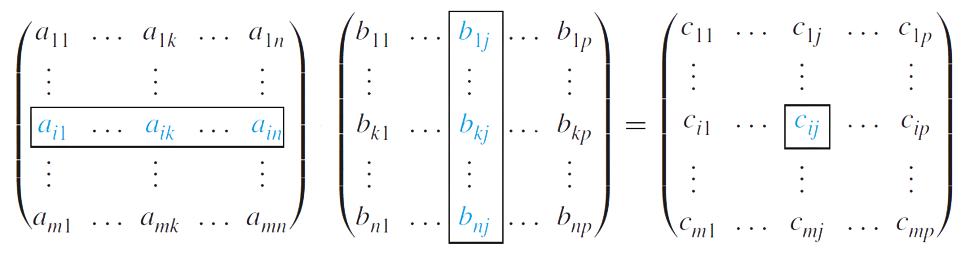
\includegraphics[width = \textwidth]{img/matrix-multiplication.png}
    
\end{frame}

\begin{frame}{Matrix multiplication. Examples}

    \begin{block}{Example}
        $$
        A =
        \begin{pmatrix}
        0 & 1  & 2 \\
        2 & 3  & 1 \\
        4 & -1 & 6 
        \end{pmatrix},\quad 
        B =
        \begin{pmatrix}
         3 & 2  \\
         1 & 0 \\
        -1 & 1
        \end{pmatrix}\quad \Longrightarrow\quad
        AB = 
        \begin{pmatrix}
        -1 & 2  \\
         8 & 5 \\
         5 & 14
        \end{pmatrix}.
        $$
        Note that $BA$ is not well defined, since the number of columns of $A$ is not equal to the number of rows of $B$.
    \end{block}

    \begin{block}{Example}
        $$
        A = 
        \begin{pmatrix}
        5  & 1  \\
        2  & 3
        \end{pmatrix},\quad
        B = \begin{pmatrix}
        1  & 2  \\
        3  & 4
        \end{pmatrix}\quad \Longrightarrow\quad
        AB = 
        \begin{pmatrix}
         8 & 14  \\
        11 & 16
        \end{pmatrix},\quad
        BA = \begin{pmatrix}
        9  & 7  \\
        33 & 15
        \end{pmatrix}.
        $$
        Note that $AB \neq BA$.
    \end{block}
    
\end{frame}

\begin{frame}{Rules of matrix multiplication}

    \begin{block}{Rules for matrix multiplication}
    Let $A$, $B$, and $C$ be matrices, and $a\in\R$. The following equalities hold, given that the matrices dimensions allow each multiplication operations to be well defined.

    \begin{minipage}{0.4\textwidth}
    \begin{enumerate}[leftmargin = 0.8cm, label = $\bullet$, rightmargin = 0.2cm]
        \item $(AB)C = A(BC)$
        \item $A(B+C) = AB + AC$
    \end{enumerate}
    \end{minipage}
    \begin{minipage}{0.4\textwidth}
    \begin{enumerate}[leftmargin = 0.8cm, label = $\bullet$, rightmargin = 0.2cm]
        \item $(A+B)C = AC + BC$
        \item $(aA) = A(aB) = a(AB)$
    \end{enumerate}
    \end{minipage}
    

    Note: Matrix multiplication is not commutative in general.
    \end{block}

    \textbf{Example}\\
        Let $A = \begin{pmatrix}
        1 & 2 \\
        0 & 1 
        \end{pmatrix}$, $B = \begin{pmatrix}
        0 & -1 \\
        3 & 2 
        \end{pmatrix}$, and $C = \begin{pmatrix}
        1 & 1 \\
        2 & 1 
        \end{pmatrix}$. Then,
        \begin{align*}
        B+C = \begin{pmatrix}
        1 & 0 \\
        5 & 3 
        \end{pmatrix} &\Longrightarrow A(B+C) = \begin{pmatrix}
        11 & 6 \\
        5 & 3 
        \end{pmatrix}\\
        AC = \begin{pmatrix}
        5 & 3 \\
        2 & 1 
        \end{pmatrix} &\Longrightarrow AB + AC = \begin{pmatrix}
        11 & 6 \\
        5 & 3 
        \end{pmatrix}.
        \end{align*}
    
\end{frame}

\begin{frame}{The identity matrix}

    \begin{block}{Identity matrix}
        A particularly useful matrix is the identity matrix (of size $n$), defined as
        $$
        I_{n} = 
        \begin{pmatrix}
        1      & 0      & \cdots & 0  \\
        0      & 1      & \cdots & 0  \\
        \vdots & \vdots &        & \vdots  \\
        0      & 0      & \cdots & 1  
        \end{pmatrix}
        $$
        The identity matrix is the equivalent of the number $1$ in the real number system, since it satisfies the relations 
        $$
        I_nA = AI_n = A
        $$
        for any $n\times n$ matrix $A$.
    \end{block}
    
\end{frame}

%----------------------- MATRICES, VECTORS, AND MATRIX ALGEBRA -----------------------%

%----------------------- SYSTEM OF LINEAR EQUATIONS -----------------------%
\section{Systems of linear equations}

\begin{frame}{System of equations in matrix form}

    \begin{enumerate}[leftmargin = 0.6cm, label = $\bullet$, rightmargin = 0.4cm]
        \item Matrix algebra is used to express system of linear equations in the packed form $A{\bf x} = {\bf b}$, where:
        \begin{enumerate}[leftmargin = 0.6cm, label = $\pmb{+}$, rightmargin = 0.4cm]
            \item $A$ is the matrix of coefficients, 
            \item ${\bf x}$ is the vector of unknowns, 
            \item ${\bf b}$ is the vector of responses.
        \end{enumerate}
         
         \medskip

        \item \textbf{Example:} \quad
        $
        \begin{aligned}
            3x_1+4x_2&=5\\
            7x_1-2x_2&=2
        \end{aligned}
        \;\Longleftrightarrow\;
        \begin{pmatrix}3&4\\7&-2\end{pmatrix}
        \begin{pmatrix}x_1\\x_2\end{pmatrix}=
        \begin{pmatrix}5\\2\end{pmatrix}
        $
        \medskip

        \item \textbf{General case:}
        $$
        \begin{pmatrix}
        a_{11} & a_{12} & \cdots & a_{1n}  \\
        a_{21} & a_{22} & \cdots & a_{2n}  \\
        \vdots & \vdots &        & \vdots  \\
        a_{m1} & a_{m2} & \cdots & a_{mn}  
        \end{pmatrix}
        \begin{pmatrix}
        x_1 \\
        x_2 \\
        \vdots \\
        x_n
        \end{pmatrix}
        =
        \begin{pmatrix}
        b_1 \\
        b_2 \\
        \vdots \\
        b_m
        \end{pmatrix}
        \Longleftrightarrow
        \begin{aligned}
            a_{11}x_1 + a_{12}x_2 + \cdots + a_{1n}x_n  &= b_1 \\
            a_{21}x_1 + a_{22}x_2 + \cdots + a_{2n}x_n  &= b_2 \\
            \vdots \hspace{1cm} \vdots \hspace{1.7cm} \vdots \hspace{0.3cm} & \hspace{0.6cm} \vdots \\
            a_{m1}x_1 + a_{m2}x_2 + \cdots + a_{mn}x_n  &= b_m
        \end{aligned}
        $$
        
    \end{enumerate}

\end{frame}

\begin{frame}{Solving linear systems. Augmented matrix and Gaussian eliminations}
\small

\begin{enumerate}[leftmargin = 0.6cm, label = $\bullet$, rightmargin = 0.4cm]
    \item \textbf{Gaussian elimination} is the process of applying elementary row operations to solve a linear system

    \item \textbf{Elementary row operations} preserve the solutions of the system. They are:
    \begin{enumerate}[leftmargin = 0.6cm, label = $\bullet$, rightmargin = 0.4cm]
        \item Swap rows,
        \item Multiply a row by a nonzero constant,
        \item Add a multiple of one row to another
    \end{enumerate}

    \item \textbf{The augmented matrix} $\pmb{A|}{\bf b}$ is used for Gaussian elimination to shorten notation

    \item \textbf{Example:} 
    \[
    \hspace{1.1cm} 
    \left[
    \begin{array}{ccc|c}
    0 & 2 & -1 & -7\\
    1 & 1 & 3  & 2\\
    -3& 2 & 2  & -10
    \end{array}
    \right]
    \;\xrightarrow{\ \hspace{0.79cm} R_1\leftrightarrow R_2 \hspace{0.79cm} \ }\;
    \left[
    \begin{array}{ccc|c}
    1 & 1 & 3  & 2\\
    0 & 2 & -1 & -7\\
    -3& 2 & 2  & -10
    \end{array}
    \right]
    \]
    \[
    \xrightarrow{\ R_3\leftarrow R_3+3R_1\ }\;
    \left[
    \begin{array}{ccc|c}
    1 & 1 & 3  & 2\\
    0 & 2 & -1 & -7\\
    0 & 5 & 11 & -4
    \end{array}
    \right]
    \xrightarrow{\ R_2\leftarrow \tfrac12 R_2,\; R_3\leftarrow R_3-5R_2\ }
    \left[
    \begin{array}{ccc|c}
    1 & 1 & 3  & 2\\
    0 & 1 & -\tfrac12 & -\tfrac72\\
    0 & 0 & \tfrac{27}{2} & \tfrac{27}{2}
    \end{array}
    \right]
    \]
    
    Back-substitution gives \(x_3=1,\ x_2=-3,\ x_1=2\).

    \item The final augmented matrix after Gaussian eliminations is called the (row) \textbf{echelon form}
\end{enumerate}

\end{frame}

\begin{frame}{Rank and solutions of a System of Linear Equation (SLE).}

    \begin{enumerate}[leftmargin = 0.6cm, label = $\bullet$, rightmargin = 0.4cm]
                
        \item The number of non-zero rows ($\neq (0 \cdots 0\, |\, 0)$) of the echelon form is called \textbf{rank of the SLE}, and usually denoted by $r$.\medskip

        \item If the echelon form has a row that looks like $(0 \cdots 0\, |\, a)$ with \(a\neq 0\), then \textbf{the SLE has no solution}, and it is said to be \textbf{inconsistent}.\medskip
        
        \item Otherwise, it is said to be \textbf{consistent}, and:
        \begin{itemize}
            \item $r=n$ \(\Rightarrow\) \textbf{unique solution};
            \item \(r<n\) \(\Rightarrow\) \textbf{infinitely many solutions} with \(n-r\) free variables (degrees of freedom),
        \end{itemize}
        where $n$ is the number of variables (columns).
        
    \end{enumerate}
    
\end{frame}

%----------------------- SYSTEM OF LINEAR EQUATIONS -----------------------%

%----------------------- SQUARE SYSTEM OF LINEAR EQUATIONS -----------------------%
\section{Square matrices}

\begin{frame}{Square matrices}
% \small

\begin{enumerate}[leftmargin = 0.6cm, label = $\bullet$, rightmargin = 0.4cm]

    \item \textbf{Square matrices} have the \textbf{same number of rows and columns} (\(n\times n\)).\medskip

    \item Viewed as a SLE, they correspond to ``same \# equations as \# unknowns''.\medskip

    \item Square matrices let us talk about \textbf{determinants} and \textbf{inverses}, which control existence and uniqueness of solutions.

\end{enumerate}

\end{frame}

\begin{frame}{Determinants}
% \small

\begin{enumerate}[leftmargin = 0.6cm, label = $\bullet$, rightmargin = 0.4cm]

    \item The determinant of a square matrix $A$ is a scalar that provides information about the linear transformation it represents.

    \item It is denoted by $|A|$.

    \item For \(A=\begin{pmatrix} a&b\\ c&d \end{pmatrix}\), the determinant is
    $
    |A|=\begin{vmatrix} a&b\\ c&d \end{vmatrix}=ad-bc.
    $

    \item \textbf{Example:}\ \(\begin{pmatrix}4&1\\3&2\end{pmatrix} \Rightarrow |A|=4\cdot2-3\cdot1=5.\)
    \item For larger matrices, the calculation becomes more complex and typically involves recursively breaking down the matrix into smaller sub-matrices until reaching the easier $2\times 2$ or $3\times 3$ cases. 

    \item We will not compute big determinants by hand. Instead, what we need is:
    \begin{align*}
        A \text{ is \textbf{invertible} } 
        &\Longleftrightarrow |A| \neq 0 \\
        &\Longleftrightarrow \text{ \textbf{unique solution}  for } A{\bf x}={\bf b} \text{ for every b }.
    \end{align*}
        

\end{enumerate}

\end{frame}


\begin{frame}{The inverse of a matrix and its use for solving SLEs}
\small
\begin{block}{Definition of inverse}
\(X\) is an inverse of \(A\) if \(AX=XA=I\). If it exists, it is unique; we write \(A^{-1}\).
\end{block}

\begin{enumerate}[leftmargin = 0.6cm, label = $\bullet$, rightmargin = 0.4cm]
    \item Not every matrix has an inverse (e.g.\ \(\begin{pmatrix}0&0\\2&1\end{pmatrix}\)).
    \medskip

    \item \textbf{In practice}, to solve \(A{\bf x}={\bf b}\) the inverse \(A^{-1}\) is not explicitly computed, as it is too computational expensive and prone to numerical instability; Gaussian elimination and other techniques are used instead.

    \item If \(A\) is invertible,
    \[
    A{\bf x}={\bf b} \ \Longleftrightarrow\ A^{-1}A{\bf x}=A^{-1}{\bf b} \ \Longleftrightarrow\ {\bf x}=A^{-1}{\bf b}.
    \]
    
    \item \(A\) is invertible \textbf{iff} for every \(b\) the system \(Ax=b\) has a \textbf{unique} solution.

    \item ${\bf 2\times2}$ \textbf{case:} If \(A=\begin{pmatrix} a&b\\ c&d \end{pmatrix}\) and \(ad-bc\neq 0\), then
    \[
    \ A^{-1}=\frac{1}{|A|}\begin{pmatrix} d&-b\\ -c&a \end{pmatrix}.
    \]

    \item \textbf{Exercise:} prove the $\bf 2\times2$ case
\end{enumerate}

\end{frame}

\section{Applications}

\begin{frame}{The Leontief (or input-output) model}

    \begin{enumerate}[leftmargin = 0.6cm, label = $\bullet$, rightmargin = 0.4cm]

        \item \textbf{The Leontief model} describes an economy with $n$ interlinked industries.
        
        \item Each industry produces a single good, using the outputs of the other industries. 

        \item \textbf{Formulation:}
        \begin{align*}
            x_i &= \text{ total number of units of good } i \text{ that the industry } i \text{ produces.} \\     
            a_{ij} &= \text{ number of units of good } i \text{ needed to produce one unit of good } j. \\
            b_i &= \text{ final demand of good } i \text{ that industry } i \text{ must satisfy }.
        \end{align*}

        \item \textbf{Demand-supply equilibrium:} 
        $$
        x_i = a_{i1}x_1 + a_{i2}x_2 + \cdots + a_{in}x_n + b_i,
        $$

        \item \textbf{SLE formulation:}\ 
        $
        (I-A){\bf x} = {\bf b},
        $
        for:
        \begin{enumerate}[leftmargin = 0.6cm, label = $\pmb{-}$, rightmargin = 0.4cm]
            \item input-output matrix $A = (a_{ij})_{n\times n}$, 
            \item production vector ${\bf x} = (x_1 \cdots x_n)'$,
            \item demand vector ${\bf b} = (b_1 \cdots b_n)'$.
        \end{enumerate}
        
        \item \textbf{Question:} Why it is reasonable to assume that $a_{ii} < 1$?
    \end{enumerate}
   
\end{frame}

\begin{frame}{The Leontief Model. An Example}

    \begin{block}{Problem}    
        Consider an economy with $n = 3$ industries: Agriculture, Manufacturing, and Energy. The production requirements are:
        \begin{itemize}
            \item[$\bullet$] $0.5$ unit of Energy per unit of Agriculture,
            \item[$\bullet$] $1$ unit of Agriculture per unit of Manufacturing,
            \item[$\bullet$] $0.5$ unit of Manufacturing per unit of Energy.
        \end{itemize}
        The final demand vector is ${\bf b}=(20\;30\;10)'$. How much must be produced?
    \end{block}

    \small
    \textbf{Solution.}
    The input–output matrix is
    \(
    A=\begin{pmatrix}
    0 & 1 & 0\\
    0 & 0 & 0.5\\
    0.5 & 0 & 0
    \end{pmatrix},
    \)
    so
    \(
    (I-A)=\begin{pmatrix}
    1 & -1 & 0\\
    0 & 1 & -0.5\\
    -0.5 & 0 & 1
    \end{pmatrix}.
    \)
    Solving $(I-A)\,{\bf x}={\bf b}$ gives
    \[
    {\bf x}=\begin{pmatrix}220/3\\[2pt] 160/3\\[2pt]140/3\end{pmatrix}
    \]
\end{frame}


\end{document}
